\documentclass[a4paper,11pt]{report}
\usepackage{chuan_math_gkt}
\usetikzlibrary{angles,quotes,intersections,patterns,decorations.pathreplacing}
\chuanexamsetup

\begin{document}
\examfontsize

\examsecret{绝密$\bigstar$启用前}

\examtitle{2020年普通高等学校招生全国统一考试（新课标I卷文科）}{数\quad 学}

\noticetitle
\begin{examnotice}
\item 答卷前，考生务必将自己的姓名、准考证号填写在答题卡上。
\item 回答选择题时，选出每小题的答案后，用铅笔把答题卡上对应题目的答案标号涂黑。如需改动，用橡皮擦干净后，再选涂其他答案标号。回答非选择题时，将答案写在答题卡上。写在本试卷上无效。
\item 考试结束后，将本试卷和答题卡一并交回。
\end{examnotice}
\examsection{一、选择题：本题共12小题，每小题5分，共60分。在每小题给出的四个选项中，只有一项是符合题目要求的。}
\begin{examquestions}

\item 已知集合A=\{x\textbar $x^{2}$-3x-4<0\}，B=\{-4，1，3，5\}，则A\ensuremath{\cap}B=

\fourchoices{\{-4，1\}}{\{1，5\}}{\{3，5\}}{\{1，3\}}

\item 若z=1+2i+$i^{3}$，则\textbar z\textbar=

\fourchoices{0}{1}{$\sqrt{2}$}{2}

\item 埃及胡夫金字塔是古代世界建筑奇迹之一，它的形状可视为一个正四棱锥。以该四棱锥的高为边长的正方形面积等于该四棱锥一个侧面三角形的面积，则其侧面三角形底边上的高与底面正方形的边长的比值为

\begin{tightcenter}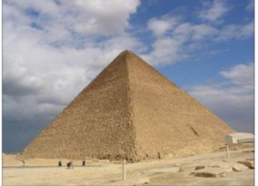
\includegraphics[width=2.6875in,height=1.9375in]{figures/2020_xkb1_wen_image3.png}\end{tightcenter}

\onechoices{$\dfrac{\sqrt{5}-1}{4}$}{$\dfrac{\sqrt{5}-1}{2}$}{$\dfrac{\sqrt{5}+1}{4}$}{$\dfrac{\sqrt{5}+1}{2}$}

\item 设O为正方形ABCD的中心，在O，A，B，C，D中任取3点，则取到的3点共线的概率为

\fourchoices{$\dfrac{1}{5}$}{$\dfrac{2}{5}$}{$\dfrac{1}{2}$}{$\dfrac{4}{5}$}

\item 某校一个课外学习小组为研究某作物种子的发芽率y和温度x(单位：$^\circ$C)的关系，在20个不同的温度条件下进行种子发芽实验，电邮实验数($x_{i}$，$y_{i}$)(i=1，2，\ensuremath{\ldots}，20)得到下面的散点图：

\begin{tightcenter}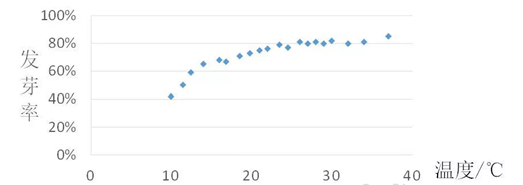
\includegraphics[width=5.44722in,height=1.92708in]{figures/2020_xkb1_wen_image12.png}\end{tightcenter}

由此散点图，在10°C至40°C之间，下面四个回归方程类型中最适宜作为发芽率y和温度x的回归方程类型的是

\fourchoices{y=a+bx}{y=a+b$x^{2}$}{y=a+b$e^{x}$}{$y=a+b\ensuremath{\ln x}$}

\item 已知圆$x^{2}$+$y^{2}$-6x=0，过点(1，2)的直线被该圆所截得的弦的长度的最小值为

\fourchoices{1}{2}{3}{4}

\item 设函数$f(x)=\cos(\omega x+\dfrac{\pi}{6})$在$[-\pi,\pi]$的图像大致如下图，则$f(x)$的最小正周期为

\begin{tightcenter}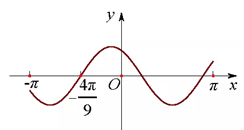
\includegraphics[width=2.54167in,height=1.35417in]{figures/2020_xkb1_wen_image14.png}\end{tightcenter}

\fourchoices{$\dfrac{10\pi}{9}$}{$\dfrac{7\pi}{6}$}{$\dfrac{4\pi}{3}$}{$\dfrac{3\pi}{2}$}

\item 设a$\log_{3}4$=2，则4\textsuperscript{-a}=

\fourchoices{$\dfrac{1}{16}$}{$\dfrac{1}{9}$}{$\dfrac{1}{8}$}{$\dfrac{1}{6}$}

\item 执行右图的程序框图，则输出的n=

\begin{tightcenter}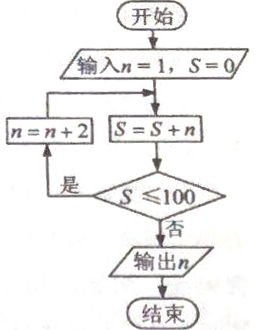
\includegraphics[width=1.44653in,height=1.8125in]{figures/2020_xkb1_wen_image23.png}\end{tightcenter}

\fourchoices{17}{19}{21}{23}

\item 设\{$a_{n}$\}是等比数列，且$a_{1}$+$a_{2}$+$a_{3}$=1，$a_{2}$+$a_{3}$+$a_{4}$=2，则$a_{6}$+$a_{7}$+$a_{8}$=

\fourchoices{12}{24}{30}{32}

\item 设$F_{1}$，$F_{2}$是双曲线C：$x^{2}-\dfrac{y^{2}}{3}=1$的两个焦点，O为坐标原点，点P在C上且\textbar OP\textbar=2，则\ensuremath{\triangle}P$F_{1}$$F_{2}$的面积为

\fourchoices{$\dfrac{7}{2}$}{3}{$\dfrac{5}{2}$}{2}

\item 已知A，B，C为球O的球面上的三个点，$\odot$$O_{1}$为\ensuremath{\triangle}ABC的外接圆，若$\odot$$O_{1}$的面积为4π，AB=BC=AC=O$O_{1}$，则球O的表面积为

\fourchoices{64π}{48π}{36π}{32π}

\item 若x，y满足约束条件\linsys{2x+y-2\ensuremath{\leq}0\\x-y-1\ensuremath{\geq}0\\y+1\ensuremath{\geq}0}，则z=x+7y的最大值为
。

\item 设向量a=(1，-1)，b=(m+1，2m-4)，若a\ensuremath{\perp}b，则m= 。

\item 曲线$y=\ensuremath{\ln x}+x+1$的一条切线的斜率为2，则该切线的方程为 。

\item 数列\{$a_{n}$\}满足$a_{n+2}$+(-1)\textsuperscript{n}$a_{n}$=3n-1，前16项和为540，则$a_{1}$=
。

\end{examquestions}
\examsection{三、解答题：共70分。解答应写出文字说明、证明过程或演算步骤。第17题～第21题为必考题，每个试题考生都必须作答。第22、23题为选考题，考生根据要求作答。}
\begin{examanswers}[start=17]


\item（12分）

某厂接受了一项加工业务，加工出来的产品(单位：件)按标准分为A，B，C，D四个等级。加工业务约定：对于A级品、B级品、C级品，厂家每件分别收取加工费90元，50元，20元；对于D级品，厂家每件要赔偿原料损失费50元。该厂有甲、乙两个分厂可承接加工业务。甲分厂加工成本费为25元/件，乙分厂加工成本费为20元/件。厂家为决定由哪个分厂承接加工业务，在两个分厂各试加工了100件这种产品，并统计了这些产品的等级，整理如下：

\begin{tightcenter}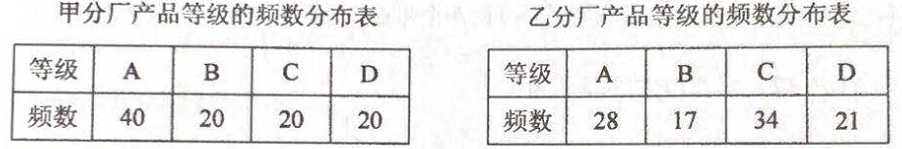
\includegraphics[width=5.75347in,height=0.95069in]{figures/2020_xkb1_wen_image28.png}\end{tightcenter}

(1)分别估计甲、乙两分厂加工出来的一件产品为A级品的概率；

(2)分别求甲、乙两分厂加工出来的100件产品的平均利润，以平均利润为依据，厂家应选哪个分厂承接加工业务?

\item（12分）

\ensuremath{\triangle}ABC的内角A，B，C的对边分别为a，b，c。已知B=150°。

(1)若a=$\sqrt{3}$c，b=2$\sqrt{7}$，求\ensuremath{\triangle}ABC的面积；

(2)若\ensuremath{\sin A}+$\sqrt{3}$\ensuremath{\sin C}=$\dfrac{\sqrt{2}}{2}$，求C。

\item（12分）

如图，D为圆锥的顶点，O是圆锥底面的圆心，\ensuremath{\triangle}ABC是底面的内接正三角形，P为DO上一点，∠APC=90°。

\begin{tightcenter}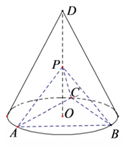
\includegraphics[width=1.38542in,height=1.52083in]{figures/2020_xkb1_wen_image32.png}\end{tightcenter}

(1)证明：平面PAB\ensuremath{\perp}平面PAC；

(2)设DO=$\sqrt{2}$，圆锥的侧面积为$\sqrt{3}$π，求三棱锥P-ABC的体积。

\item（12分）

已知函数f(x)=$e^{x}$-a(x+2)，

(1)当a=1时，讨论f(x)的单调性；

(2)若f(x)有两个零点，求a的取值范围。

\item（12分）

已知函数f(x)=$e^{x}$+a$x^{2}$-x。

(1)当a=1时，讨论f(x)的单调性；

(2)当x\ensuremath{\geq}0时，f(x)\ensuremath{\geq}$\dfrac{1}{2}$$x^{3}$+1，求a的取值范围。


\item（10分）

{[}选修4-4：坐标系与参数方程{]}(10分)

在直角坐标系xOy中，曲线$C_{1}$的参数方程为\linsys{x=\cos^kt\\y=\sin^kt}
(t为参数)。以坐标原点为极点，x轴正半轴为极轴建立极坐标系，曲线$C_{2}$的极坐标方程为4ρcosθ-16ρsinθ+3=0。

(1)当k=1时，$C_{1}$是什么曲线?

(2)当k=4时，求$C_{1}$与$C_{2}$的公共点的直角坐标。

\item（10分）

{[}选修4-5：不等式选讲{]}(10分)

已知函数f(x)=\textbar3x+1\textbar-2\textbar x-1\textbar。

\begin{tightcenter}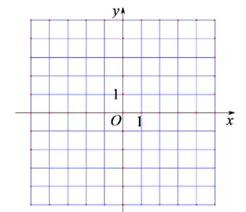
\includegraphics[width=2.5625in,height=2.20833in]{figures/2020_xkb1_wen_image35.png}\end{tightcenter}

(1)画出y=f(x)的图像；

(2)求不等式f(x)> f(x+1)的解集。
\end{examanswers}

\end{document}
